\subsection{Sprint 13: da 2024-09-02 a 2024-09-15}
\par Poiché i test di unità, integrazione e sistema sono stati completati, nello \glossario{sprint} 13 il team si dedicherà alla fase di collaudo. I risultati dei test di accettazione verranno registrati nel \PdQ, che sarà aggiornato anche nel cruscotto di valutazione della qualità. Inoltre, il gruppo amplierà il documento di \ST, verificando al contempo il codice sorgente.

\subsubsection{Obiettivi}
\begin{itemize}
  \item Aggiornamento metriche nelle \NdP;
  \item Stesura verbali interni ed esterni;
  \item Consuntivo \glossario{sprint} 12;
  \item Ultimazione del cruscotto di valutazione della qualità;
  \item Implementazione di test \glossario{front-end} per migliorare la copertura del codice;
  \item Revisione completa del codice sorgente;
  \item Ampliamento del documento di \ST;
  \item Inizio fase di collaudo;
  \item Organizzazione di un incontro con la \glossario{Proponente};
  \item Integrazione Codecov-GitHub;
  \item Aggiornamento documentazione (\PdP, \NdP, \PdQ, \Gls, \MU\ e \ST).
\end{itemize}

\begin{figure}[H]
  \centering
  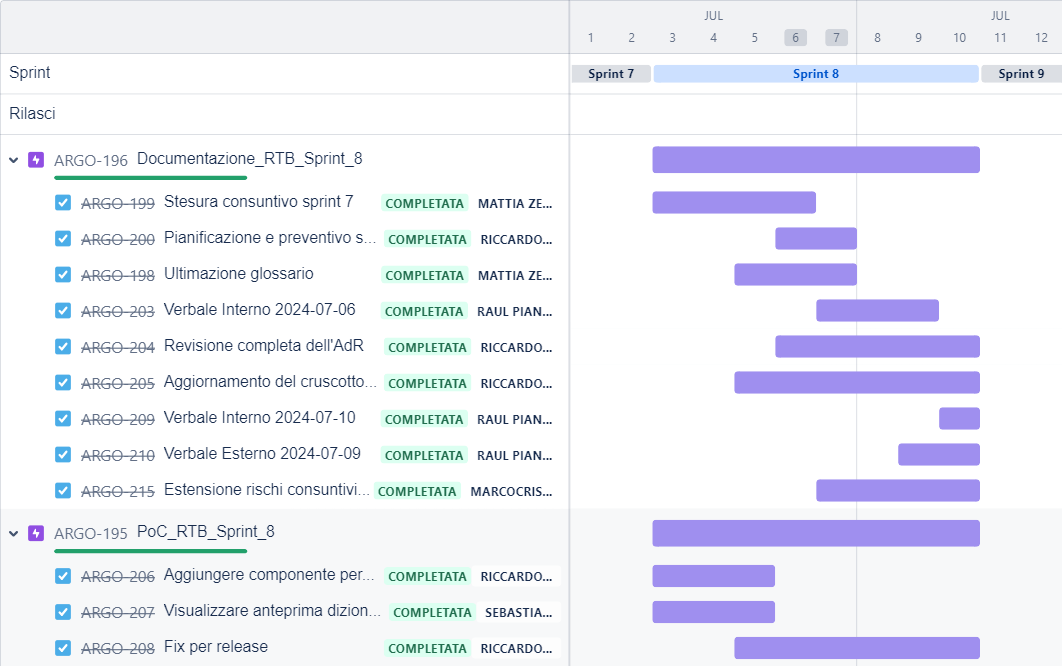
\includegraphics[width=0.90\textwidth]{assets/Pianificazione/Sprint-13/gantt.png}
  \caption{Sprint 13 - Diagramma di Gantt}\label{fig:sprint-13-gantt}
\end{figure}

